%PREAMBLE
\begin{comment}
%\documentclass[11pt]{article}
%\newcommand{\pablo}[1]{\textcolor{blue}{{\bf  #1}}}
\newcommand{\carlos}[1]{\textcolor{red}{{\bf  #1}}}
\newcommand{\fabio}[1]{\textcolor{purple}{{\bf  #1}}}
\newcommand{\susana}[1]{\textcolor{violet}{{\bf  #1}}}

% HEP names :: https://ctan.javinator9889.com/macros/latex/contrib/hepnames/hepnames.pdf

\DeclarePairedDelimiter\bra{\langle}{\rvert}
\DeclarePairedDelimiter\ket{\lvert}{\rangle}
\DeclarePairedDelimiterX\braket[2]{\langle}{\rangle}{#1 \delimsize\vert #2}

\newcommand*{\yt}{\ensuremath{y_{t}}\xspace}
\newcommand*{\tchannel}{\ensuremath{t\text{-channel}}\xspace}
\newcommand*{\schannel}{\ensuremath{s\text{-channel}}\xspace}
%\newcommand*{\lepT}{\ensuremath{\Pl_{\Pt}}\xspace}
%\newcommand*{\lepH}{\ensuremath{\Pl_{\PHiggs}}\xspace}

%\newcommand*{\muR}{\ensuremath{\mu_{\text{R}}}\xspace}
%\newcommand*{\muF}{\ensuremath{\mu_{\text{F}}}\xspace}

% Add external packages
\usepackage[italic]{hepnicenames}

%%%%%%%%%%%%%%%%%%%%%%%
%  From NA-HIGG-2020-02-INT1-defs.sty    %
%%%%%%%%%%%%%%%%%%%%%%%
% Basic tHq-related macros
%\newcommand*{\tHq}{\ensuremath{\Pqt{}\PH{}\Pq}\xspace}
%\newcommand*{\tHq}{\ensuremath{\Ptop \PHiggs \Pq}\xspace}
%\newcommand*{\tHq}{\Pqt{}\PH{}\Pq}
\newcommand*{\tHq}{\ensuremath{tHq}\xspace}
\newcommand*{\tH}{\ensuremath{\Pqt{}\PH{}}\xspace}
\newcommand*{\tHqsec}{\texorpdfstring{\Pqt{}\PH{}\Pq}{tHq}}
\newcommand*{\tHqML}{\ensuremath{\Pqt{}\PH{}\Pq\,(\text{ML})}\xspace}
\newcommand*{\tHqbb}{\ensuremath{\Pqt{}\PH{}\Pq\,(\bbbar)}\xspace}
\newcommand*{\tbarHq}{\Paqt{}\PH{}Pq}
\newcommand*{\tHbb}{\ensuremath{\tHq (\PH \to \bbbar)}\xspace}
\newcommand*{\tHtautau}{\ensuremath{\tHq (\PH \to \Pgt{}\Pgt)}\xspace}
\newcommand*{\dR}{\ensuremath{\Delta R}\xspace}
\newcommand*{\trexfitter}{TRExFitter\xspace}
\newcommand*{\thqloop}{\texttt{tHqLoop}\xspace}


\newcommand*{\MpT}{\ensuremath{\vec{p}_{\text{T}}^{\text{miss}}}\xspace}
\newcommand*{\mtw}{\ensuremath{m_{\text{T}}(\Pl,\MET)}}
\newcommand*{\mlb}{\ensuremath{m_{\Pl\Pqb}}}
\newcommand*{\mOSSF}{\ensuremath{m_{\text{OSSF}}}\xspace}

% Background processes
\newcommand*{\ttX}{\ensuremath{\Pqt{}\Paqt{}X}\xspace}
\newcommand*{\tX}{\ensuremath{\Pqt{}X}\xspace}

%\newcommand*{\ttX}{\Pqt{}\Paqt{}+X}
\newcommand*{\ttH}{\Pqt{}\Paqt{}\PH}
%\newcommand*{\ttH}{\ensuremath{\Pqt{}\Paqt{}\PH}\xspace}
\newcommand*{\ttZ}{\Pqt{}\Paqt{}\PZ}
\newcommand*{\ttV}{\ensuremath{\Pqt{}\Paqt{}V}\xspace}
\newcommand*{\ttW}{\Pqt{}\Paqt{}\PW}
\newcommand*{\ttWj}{\ensuremath{t\bar{t}W+j}\xspace}
\newcommand*{\tZq}{\Pqt{}\PZ{}\Pq}
\newcommand*{\tWZ}{\Pqt{}\PW{}\PZ}
\newcommand*{\tWH}{\Pqt{}\PW{}\PH}
\newcommand*{\tHW}{\Pqt{}\PW{}\PH}
\newcommand*{\tW}{\Pqt{}\PW}
\newcommand*{\Wt}{\Pqt{}\PW}
\newcommand*{\diboson}{diboson\xspace}
\newcommand*{\Diboson}{Diboson\xspace}
\newcommand*{\triboson}{triboson\xspace}
\newcommand*{\Triboson}{Triboson\xspace}
\newcommand*{\Vjets}{\ensuremath{V\text{+\,jets}}\xspace}

\newcommand*{\ttt}{\ensuremath{ttt}\xspace}
\newcommand*{\tttt}{\ensuremath{t\bar{t}t\bar{t}}\xspace}
\newcommand*{\ggH}{\ensuremath{ggH}\xspace}
\newcommand*{\qqH}{\ensuremath{qqH}\xspace}
\newcommand*{\WH}{\ensuremath{WH}\xspace}
\newcommand*{\ZH}{\ensuremath{ZH}\xspace}

% Fake leptons
\newcommand*{\elHF}{\ensuremath{e_{\text{HF}}}\xspace}
\newcommand*{\muHF}{\ensuremath{\mu_{\text{HF}}}\xspace}
\newcommand*{\elCo}{\ensuremath{e_{\text{conv}}}\xspace} 
\newcommand*{\kelHF}{\ensuremath{\mu(e_{\text{HF}})}\xspace}
\newcommand*{\kmuHF}{\ensuremath{\mu(\mu_{\text{HF}})}\xspace}
\newcommand*{\kelCo}{\ensuremath{\mu(e_{\text{conv}})}\xspace} 

% Signal regions
\newcommand*{\dileptau}{\ensuremath{2\Pl+1\tauhad}\xspace}
\newcommand*{\dilepOStau}{\ensuremath{2\Pl\,\text{OS}+1\tauhad}\xspace}
\newcommand*{\dilepSStau}{\ensuremath{2\Pl\,\text{SS}+1\tauhad}\xspace}

\newcommand*{\onelep}{\ensuremath{1\Pl}\xspace}
\newcommand*{\dilep}{\ensuremath{2\Pl}\xspace}
\newcommand*{\dilepOS}{\ensuremath{2\Pl\,\text{OS}}\xspace}
\newcommand*{\dilepSS}{\ensuremath{2\Pl\,\text{SS}}\xspace}
%\newcommand*{\SS}{\ensuremath{\text{SS}}\xspace}
%\newcommand*{\OS}{\ensuremath{\text{OS}}\xspace}

\newcommand*{\trilep}{\ensuremath{3\Pl}\xspace}
\newcommand*{\lepditau}{\ensuremath{1\Pl+2\tauhad}\xspace}




\newcommand*{\lumi}{\ensuremath{\mathcal{L}}\xspace}
\newcommand*{\lumiunits}{$\,$ cm$^{2} \,$s$^{-1}$\xspace}


%Other
\newcommand*{\CM}{\ensuremath{\sqrt{s}}\xspace}
 
\newcommand*{\Wtb}{\ensuremath{tWb}\xspace}
\newcommand*{\tWb}{\Wtb}
%\newcommand*{\tWb}{\ensuremath{tWb}\xspace}
\newcommand*{\pfour}{\ensuremath{\boldsymbol{\textrm{p}}}\xspace} 

\newcommand*{\tchan}{\ensuremath{t}-channel}
\newcommand*{\mtop}{\ensuremath{m_{\Ptop}}\xspace}
%\newcommand*{\mH}{\ensuremath{m_H}\xspace}
%\newcommand*{\HT}{\ensuremath{H_{\text{T}}}\xspace}

%\newcommand*{\PWplus}{\ensuremath{\PW^{+}}\xspace}
%\newcommand*{\PWminus}{\ensuremath{\PW^{-}}\xspace}
%\newcommand*{\Pgamma}{\ensuremath{\gamma}\xspace}

 \newcommand*{\greekphys}{\ensuremath{\varphi\upsilon\sigma\iota\kappa \eta}\xspace}
 \newcommand*{\greekatom}{\ensuremath{\alpha \tau o \mu o \nu}\xspace}
 \newcommand{\emu}{\ensuremath{\Pe/\Pmu}\xspace}

\newcommand*{\momentum}{\ensuremath{\overrightarrow{p}}\xspace} 
%\newcommand*{\CP}{\ensuremath{\mathcal{CP}}\xspace}
\newcommand*{\CP}{CP\xspace}

% Decays (Please, check latex/atlasprocess.sty and latex/atlasparticle.sty for more definitions!)
\newcommand{\bb}{\ensuremath{\Pqb\Paqp}\xspace}
\newcommand{\WW}{\ensuremath{\PW\PW^{*}}\xspace}
\newcommand{\ZZ}{\ensuremath{\PZ\PZ^{*}}\xspace}
\newcommand{\Higgsdecays}{\ensuremath{\PH \rightarrow b\bar{b}, \WW, \ZZ, \tau\tau}\xspace}
\newcommand{\Higgsdecayslep}{\ensuremath{\PH \rightarrow \WW, \ZZ, \tau\tau}\xspace}
\newcommand{\HWW}{\ensuremath{\PH \rightarrow \WW}\xspace}
\newcommand{\HZZ}{\ensuremath{\PH \rightarrow \ZZ}\xspace}

% reconstruction definitions
\newcommand{\pnutop}{\ensuremath{\vec{p^{\Pnu, \text{top}}}}\xspace}
\newcommand{\pnutopx}{\ensuremath{p^{\Pnu, \text{top}}_x}\xspace}
\newcommand{\pnutopy}{\ensuremath{p^{\Pnu, \text{top}}_y}\xspace}
\newcommand{\pnutopz}{\ensuremath{p_{z}(\Pnu_{\text{top}})}\xspace}
\newcommand{\pnutopT}{\ensuremath{\pT(\Pnu_{\text{top}})}\xspace}
\newcommand{\phinutop}{\ensuremath{\phi(\Pnu_{\text{top}})}\xspace}
\newcommand{\pltop}{\ensuremath{\vec{p^{\Plepton, \text{top}}}}\xspace}
\newcommand{\pltopx}{\ensuremath{p^{\Plepton, \text{top}}_x}\xspace}
\newcommand{\pltopy}{\ensuremath{p^{\Plepton, \text{top}}_y}\xspace}
\newcommand{\pltopz}{\ensuremath{p^{\Plepton, \text{top}}_z}\xspace}
\newcommand{\pltopT}{\ensuremath{\pT(\Plepton_{\text{top}})}\xspace}
\newcommand{\philtop}{\ensuremath{\phi(\ell_{\text{top}})}\xspace}
\newcommand{\phibtop}{\ensuremath{\phi(b_{\text{top}})}\xspace}
\newcommand{\tauvis}{\ensuremath{\Ptau_{\text{vis}}}\xspace}

\newcommand{\leptop}{\ensuremath{\Plepton^{\text{top}}}\xspace}
\newcommand{\lepH}{\ensuremath{{\Plepton^{\PH}}}\xspace}
\newcommand{\Hvismass}{\ensuremath{m_{\PH}^{\text{vis}}}\xspace}
\newcommand{\toprecomass}{\ensuremath{\mtop^{\text{reco}}}\xspace}
% \newcommand{\toprecomass}{\ensuremath{\Pqt_{\text{reco}}^{\text{m}}\xspace}}
% \newcommand{\Hvismass}{\ensuremath{\PH_{\text{vis}}^{\text{m}}\xspace}}
\newcommand{\MMC}{\texttt{MissingMassCalculator}\xspace}

% luminosity (2015)
\newcommand{\lumiFifteenRelUnc}{1.13} % in [%]
\newcommand{\lumitagFifteen}{{\small\texttt{OfLumi-13TeV-008}}}
%\newcommand{\lumiFifteenInPbNoUnits}{3219.56}
%\newcommand{\lumiFifteenInFbNoUnits}{3.2}
\newcommand{\lumiFifteenInPbNoUnits}{3244.54} % final luminosity recommendation for Run 2 analyses (https://twiki.cern.ch/twiki/bin/viewauth/Atlas/LuminosityForPhysics#2015_2018_13_TeV_proton_proton_f)
\newcommand{\lumiFifteenInFbNoUnits}{3.2}
%\newcommand{\dataperiodsFifteen}{D--J}
\newcommand{\dataperiodsFifteen}{D--H,J}
\newcommand{\firstdatarunFifteen}{276262}
\newcommand{\lastdatarunFifteen}{284484}
\newcommand{\datarunsFifteen}{\firstdatarunFifteen--\lastdatarunFifteen}
\newcommand{\dataeventsFifteen}{220.58M}

% luminosity (2016)
\newcommand{\lumiSixteenRelUnc}{0.89} % in [%]
\newcommand{\lumitagSixteen}{{\small\texttt{OfLumi-13TeV-009}}}
%\newcommand{\lumiSixteenInPbNoUnits}{32988.1}
%\newcommand{\lumiSixteenInFbNoUnits}{33.0}
% final luminosity recommendation for Run 2 analyses (https://twiki.cern.ch/twiki/bin/viewauth/Atlas/LuminosityForPhysics#2015_2018_13_TeV_proton_proton_f)
\newcommand{\lumiSixteenInPbNoUnits}{33402.2}
\newcommand{\lumiSixteenInFbNoUnits}{33.4}
%\newcommand{\dataperiodsSixteen}{A--L}
\newcommand{\dataperiodsSixteen}{A--G,I,K,L}
\newcommand{\firstdatarunSixteen}{297730}
\newcommand{\lastdatarunSixteen}{311481}
\newcommand{\datarunsSixteen}{\firstdatarunSixteen--\lastdatarunSixteen}
\newcommand{\dataeventsSixteen}{1057.84M}

% luminosity (2017)
\newcommand{\lumiSeventeenRelUnc}{1.13} % in [%]
\newcommand{\lumitagSeventeen}{{\small\texttt{OfLumi-13TeV-010}}}
%\newcommand{\lumiSeventeenInPbNoUnits}{44307.4}
%\newcommand{\lumiSeventeenInFbNoUnits}{44.3}
% final luminosity recommendation for Run 2 analyses (https://twiki.cern.ch/twiki/bin/viewauth/Atlas/LuminosityForPhysics#2015_2018_13_TeV_proton_proton_f)
\newcommand{\lumiSeventeenInPbNoUnits}{44630.6}
\newcommand{\lumiSeventeenInFbNoUnits}{44.6} 
%\newcommand{\dataperiodsSeventeen}{B--K}
\newcommand{\dataperiodsSeventeen}{B--F,H,I,K}
\newcommand{\firstdatarunSeventeen}{325713}
\newcommand{\lastdatarunSeventeen}{340453}
\newcommand{\datarunsSeventeen}{\firstdatarunSeventeen--\lastdatarunSeventeen}
%%%\newcommand{\datarunsSeventeen}{324320--341649}
\newcommand{\dataeventsSeventeen}{1340.80M}

% luminosity (2018)
\newcommand{\lumiEightteenRelUnc}{1.10} % in [%]
\newcommand{\lumitagEightteen}{{\small\texttt{OfLumi-13TeV-010}}}
%\newcommand{\lumiEightteenInPbNoUnits}{58450.1}
%\newcommand{\lumiEightteenInFbNoUnits}{58.5}
% final luminosity recommendation for Run 2 analyses (https://twiki.cern.ch/twiki/bin/viewauth/Atlas/LuminosityForPhysics#2015_2018_13_TeV_proton_proton_f)
\newcommand{\lumiEightteenInPbNoUnits}{58791.6}
\newcommand{\lumiEightteenInFbNoUnits}{58.8}
\newcommand{\lumiEightteenInPb}{\SI{\lumiEightteenInPbNoUnits}{\per\pb}}
\newcommand{\lumiEightteenInFb}{\SI{\lumiEightteenInFbNoUnits}{\per\fb}}
%\newcommand{\dataperiodsEightteen}{B--Q}
\newcommand{\dataperiodsEightteen}{B--D,F,I,K,L,M,O,Q}
\newcommand{\firstdataruEightteen}{348885}
\newcommand{\lastdatarunEightteen}{364292}
\newcommand{\datarunsEightteen}{\firstdataruEightteen--\lastdatarunEightteen}
%%%\newcommand{\datarunsEightteen}{348197--364292}
\newcommand{\dataeventsEightteen}{1716.77M}

% luminosity (2015+2016+2017)
%\newcommand{\lumiInPb}{80515.06~\invpb}
% \newcommand{\partlumi}{\SI{80.52}{\per\fb}}
%\newcommand{\datafirstyear}{2015}
%\newcommand{\datalastyear}{2017}

% luminosity (2015+2016+2017+2018)
%
% https://twiki.cern.ch/twiki/bin/viewauth/Atlas/LuminosityForPhysics#2015_2018_13_TeV_proton_proton_f
% final luminosity recommendation for Run 2 analyses (central value + uncertainty)
\newcommand{\lumiRelUnc}{0.83} % in [%]
\newcommand{\lumiInPbNoUnits}{140068.94} % in pb-1
\newcommand{\lumiInFbNoUnits}{140} % in fb-1
\newcommand{\lumiWithUnc}{\ensuremath{140.1 \pm 1.2}\,\si{\per\fb}} % in fb-1
%
% old recommendation
%\newcommand{\lumiRelUnc}{1.7} % in [%]
%\newcommand{\lumiInPbNoUnits}{138965.16} % in pb-1
%\newcommand{\lumiInFbNoUnits}{139} % in fb-1
%\newcommand{\lumiWithUnc}{\ensuremath{\lumiInFbNoUnits \pm 2.4}\,\si{\per\fb}} % in fb-1
\newcommand{\dataeventsAll}{4335.99M}
%
\newcommand{\lumiInPb}{\SI{\lumiInPbNoUnits}{\per\pb}}
%\newcommand{\lumi}{\SI{\lumiInFbNoUnits}{\per\fb}}
\newcommand{\datafirstyear}{2015}
\newcommand{\datalastyear}{2018}

% % tunes and PDF sets
\def\cteq{CTEQ6L1\xspace}
\def\ctten{CT10\xspace}
\def\cttennlo{CT10\,NLO\xspace}
\def\cttennnlo{CT10\,NNLO\xspace}
\def\ctfourteennlo{CT14\,NLO\xspace}
\def\ctfourteennnlo{CT14\,NNLO\xspace}
\def\nnpdfnnlo{NNPDF3.0\,NNLO\xspace}
\def\nnpdfnlofourflav{NNPDF3.0\,NLO\,nf4\xspace}
\def\nnpdfnlo{NNPDF3.0\,NLO\xspace}
\def\nnpdftwonlo{NNPDF2.3\,NLO\xspace}
\def\nnpdftwo{NNPDF2.3\,LO\xspace}
\def\nnpdftwofiveflav{NNPDF2.3\,5f\,FFN\xspace}
\def\mstw{MSTW2008\,NLO\xspace}
\def\a14{A14\xspace}
\def\auet{AUET2\xspace}
\def\aznlo{AZNLO\xspace}
\def\mmhtnnlo{MMHT2014\,NNLO\xspace}
\def\mmhtnlo{MMHT2014\,NLO\xspace}
\def\mmhtlo{MMHT2014\,LO\xspace}
\def\mstwnlo{MSTW2008\,68\%\,CL\,NLO \xspace}
\def\mstwnnloninety{MSTW2008\,90\%\,CL\,NNLO \xspace}
\def\ueee{UE-EE-5\xspace}




 
\endinput


%\begin{document}
asdf
%ENDPREAMBLE
\end{comment}

\chapter{Recording data and simulating events in ATLAS}
%{\LARGE \textbf{}\\}
% The content of this section has to be general, i.e. it is valid for both the polarisation and the tHq analyses
%\tableofcontents
\label{chap:DataAndMC}

\vspace*{0.1 cm} 
\hspace*{200pt} \\
\hspace*{120pt} \textit{In God we trust, all others bring data.} \\
%\hspace*{200pt} \textit{} \\
%\hspace*{200pt} \\
\hspace*{140pt} ---\textsc{William Edwards Deming (1900-1993)} \\% \textit{} \\
%\hspace*{200pt} \textit{Please check your e-mailing list} \\
\vspace*{2cm} 


The word ``event'' is one of the most commonly used terms in high energy physics.
In the context of LHC experiments there are two types of events. On side, there
are the real events recorded by the detector. This event is typically a 
$\Pproton \Pproton$ collision but it could also be a single particle such as
cosmic ray. On the other side, there the events simulated by the MC 
event generator. In ATLAS, both type of events are precessed by a common
software, Athena.
For real-collision data, the detector response is evaluated via different algorithms
in order to reconstruct the objects in the final state. For the simulated processes,
the MC generated particles undergo a serie of steps replicating the physics of
the collisions, the interaction with the detector material, the magnetic fields and
the response of the detector electronics. Once this steps have been applied,
the simulated events are evaluated using the same algorithms as the ones 
from real collisions.



 This chapter is dived is two sections that discuss both types of 
 events. While in Section \ref{sec:Chap3.1:Data} the collection of the 
 data in ATLAS is briefly described, Section \ref{sec:Chap3.1:MC}
discuses the MC simulation chain. \pablo{Ahora tmbn está la sección de pheno.}





%%%%%%%%%%%%%%
%          PP Collisions        %
%%%%%%%%%%%%%%
\section{Phenomenology of proton-proton collisions}
\label{sec:Chap2:PhenoOfPP}
During the data tracking period of LHC Run-2, proton collisions took place with a centre-of-mass energy of 13$\,$TeV. 
The total cross section for $\Pproton\Pproton$ collisions at this energy was measured to be $\sigma_{tot} = (110.6 \pm 3.4)\,$
mb according to \cite{Cafagna:2021sge}. The method used to measure $\sigma_{tot}$ also made it 
possible to separate the cross section into the elastic cross-section $\sigma_{el} = (31.9 \pm 1.7)\,$mb and 
the inelastic cross-section $\sigma_{inel} = (79.5 \pm 1.8)\,$mb.
%The inelastic cross-section is the sum of the non-diffractive and the diffractive cross-section. 
However, only inelastic scattering generates particles with an sufficient angle with respect to the beam 
axis so that these particles enter into the geometrical acceptance of the detector. 
Figure \ref{fig:Chap2:pp_cross_section_pdg} shows the cross-section (elastic, inelastic and total) for $\Pproton \Pproton$ collisions depending on \CM.
 The shown cross-section can be computed as the convolution of parton density functions (PDFs) with the parton scattering matrix element $\mathcal{M}$. 
%(the matrix element,$\mathcal{M}$, was already introduced in section \ref{sec:Chap1:tH}).

\begin{figure}
 	 \centering
 	  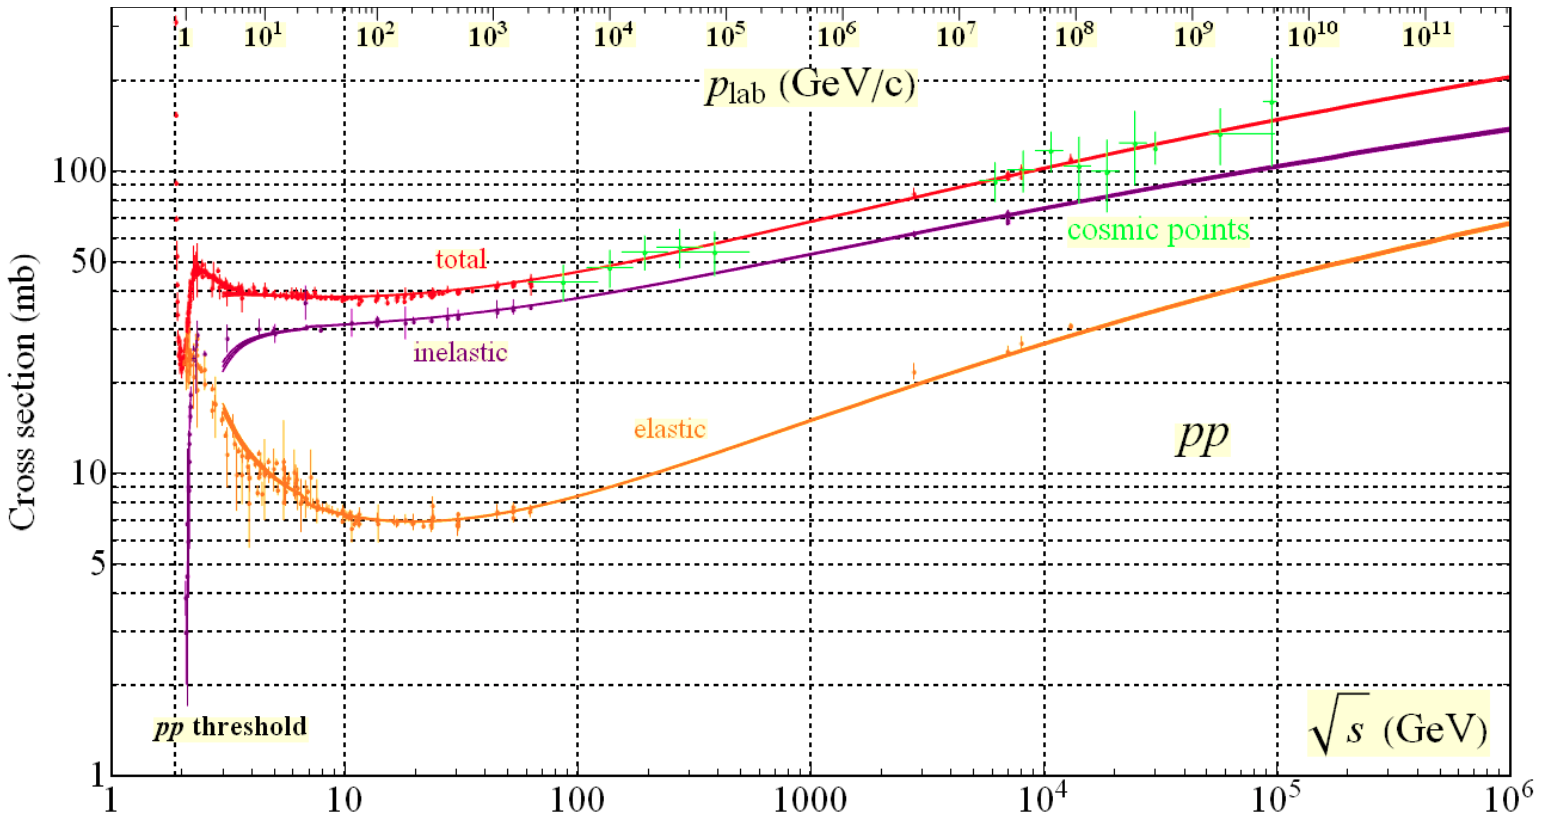
\includegraphics[width = 0.7\textwidth]{Chapter2/pp_cross_section_pdg}
	  \caption{Total and elastic cross-section for $\Pproton \Pproton$ collisions as a 
	  		function of the laboratory momentum and the $\CM$ \cite{pdgXsecProton}.
			At $\CM=13\,$TeV,  $\sigma_{el} = (31.9 \pm 1.7)\,$m, $\sigma_{inel} = (79.5 \pm 1.8)\,$mb and 
			$\sigma_{tot} = (110.6 \pm 3.4)\,$mb.} 
	\label{fig:Chap2:pp_cross_section_pdg}% source: https://pdg.lbl.gov/1998/hadronicrpp_page13.pdf
\end{figure}


At LHC energy regime,
the $\Pproton \Pproton$ collisions cannot be
described as a point-like interactions, here is where the PDFs come into play.
The PDFs are functions containing the long distance structure of the hadron in terms of valence and sea quarks and gluons. 
%More information about PDFs and the proton structure can be found in Section \ref{sec:Chap2:PhenoOfPP:ProtonStructure}.
This description is known as ``parton model''.

%See: https://arxiv.org/pdf/1611.07864.pdf
% https://indico.cern.ch/event/760184/contributions/3290951/attachments/1832936/3002261/rojo-SMLHC-PDFrev.pdf


%%%%%%%%%%%%%%%%
%           Proton structure        %
%%%%%%%%%%%%%%%%
\subsection{Proton structure and parton model for collisions}
\label{sec:Chap2:PhenoOfPP:ProtonStructure}

\begin{minipage}{.45\textwidth}
%\begin{figure}
 	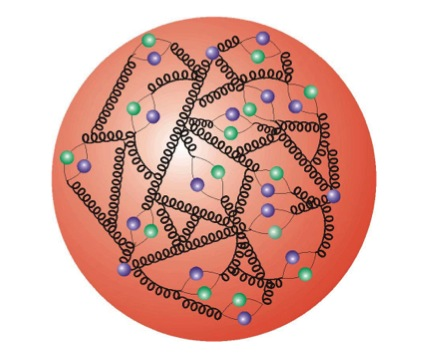
\includegraphics[width = \textwidth]{Chapter2/PartonCompositionOfHadron}
%	\caption{Content of a hadron in the parton model. For baryons like the proton there are 3 valence quarks, many virtual quark and anti-quarks pairs (sea quarks) and many gluons.}
%	\label{fig:Chap2:PartonComposition}
%\end{figure}
\end{minipage}\hfill
\begin{minipage}{.54\textwidth}
	The parton model for hadrons describes these non-fundamental particles as a composite of a number of point-like constituents named partons.
	The proton is not only simply made of three quarks ($\Pup \Pup \Pdown$, the so called ``valence'' quarks) but also, there is a ``sea'' of
	gluons and short-lived quark and anti-quark pairs. The partons in the sea are continuously interacting with each other and can have
	any flavour.
\end{minipage}


%The parton distribution functions (PDFs) are density functions that describe probability to find a parton carrying a fraction $x$
%of the total proton momentum at a squared energy scale $Q^2$. 
%The PDFs describe the distribution of the hadron's momentum among its constituents\cite{Butterworth:2015oua}.
%The momentum distribution function of the partons within the proton is obtained by a fit on a large number of cross-section data points
%over a grid of $x$ and $Q^2$ values obtained from many experiments (deep inelastic scattering, Drell-Yan and jet measurements).
%There are various global fitting collaborations (ABM, CT, MMHT, NNPDF, MSTW, CTEQ),
%each taking different approaches to this fitting procedure.  These fits are later extrapolated to new energy scales. %Several collaborations
%work on providing the PDFs sets (CT14, MMHT2014, NNPDF30, ...)
%The most relevant uncertainties associated with the computation of PDFs are the experimental uncertainties of the
%input datasets and the theoretical uncertainties of the coupling parameters. 

%Formally, the PDF $f_{a/A}(x, Q^{2})$ is defined as the probability of finding
%a parton $a$ within the hadron $A$ carrying a fraction $x=p_{a}/p_{A}$ of its momentum at $Q^{2}$ energy scale.
%The energy scale $Q$ characterises the hard scattering and typically corresponds to the momentum transfer in the given process.
%As an example, several PDFs at two different scale energies  are presented in Figure \ref{fig:Chap2:NNLO_PDF} as a function of $x$.

The distribution of a hadron's momentum among its constituents is described by its
PDFs \cite{Butterworth:2015oua}. The momentum of the partons within a proton is 
determined through fits to several cross-section data points obtained from experiments 
such as deep inelastic scattering, Drell-Yan, and jet measurements. Several global fitting 
collaborations, including ABM, CT, MMHT, NNPDF, MSTW, and CTEQ, use different 
methods to perform these fits. The fits are then extrapolated to new energy scales.

The PDF $f_{a/A}(x, Q^{2})$ is the probability of finding parton $a$ in hadron $A$ 
carrying a fraction $x=p_{a}/p_{A}$ of its momentum at the energy scale $Q^2$. 
At lower energies ($Q\sim1,$GeV), the momentum of a proton is primarily shared 
among its valence quarks, while at higher energies ($1 <Q \lesssim 1,$GeV), 
the emission of gluons carrying some of the quark's initial momentum is more likely.
As an example, several PDFs at two different scale energies  are presented in Figure \ref{fig:Chap2:NNLO_PDF} as a function of $x$
In QCD theory, these interactions can be divided into two categories: 
hard (large momentum transfer) and soft (low momentum transfer). 
Hard processes are well understood and can be predicted with good precision,
while soft interactions have a much greater impact of non-perturbative QCD and are more difficult to calculate.

\begin{figure}
 	  \centering
	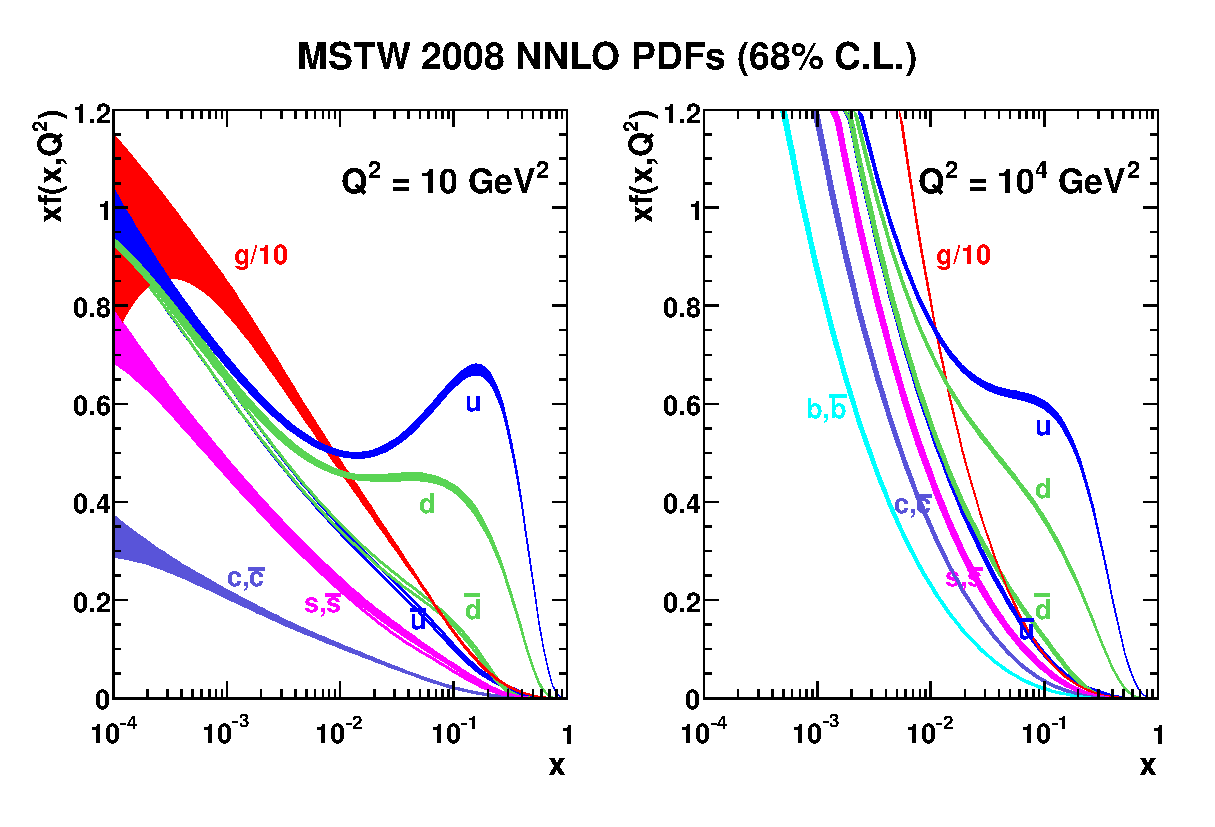
\includegraphics[width = \textwidth]{Chapter2/PDF_mstw2008nnlo68cl_allpdfs}
	\caption{Parton distribution functions $xf(x,q^{2})$ plotted against $x$ for gluons different quark flavours 
		      at $Q^{2}=10\,$GeV$^2$ and $Q^{2}=10^{4}\,$GeV$^2$ using MSTW 2008 NNLO
		      \cite{Martin:2009iq}.}
	\label{fig:Chap2:NNLO_PDF}
\end{figure} 

%The momentum of the proton is distributed among its constituents and, while at lower energies ($Q\sim1\,$GeV) it is shared mainly between the 
%valence quarks, at higher energies ($1 <Q \lesssim 1\,$GeV) the emission of gluons carrying a some of the initial momentum of the quark is more probable.
%Within the QCD theory, these interactions can be classified in two main groups: ``hard'' and ``soft''. The hard processes are those involving large 
%momentum transfer.  This type of processes are well understood and their cross-section can be predicted with good precision using perturbation theory.
%In contrast, the low momentum transfer of soft interactions leads to a much more dominant impact of non-perturbative QCD, which makes much more difficult to
%calculate the cross-section. 

When two protons ($A$ and $B$) collide, the partons of the two protons interact via a hard
scattering process. Each of the interactions between the partons pairs  is independent 
from the interactions of other partons. The remaining partons also contribute to the final state as ``underlying events''.  
Figure \ref{fig:Chap2:ProtonProton_Collision} provides a simplified representation of a $\Pproton \Pproton$ collision.

The total cross section in a hadron-hadron (where parton $a$ from hadron $A$ interacts with parton $b$ from 
hadron $B$) hard scattering process, such as a $\Pproton \Pproton$ interaction, is:
\begin{equation}
	\sigma_{AB \rightarrow X} = \sum_{a, b} \iint dx_{a} dx_{b} f_{a}(x_{a}, Q^{2})  f_{b}(x_{b}, Q^{2}) \times \hat{\sigma}_{ab\rightarrow X}
\end{equation}
where $f_{i}(x_{i}, Q^{2})$ is the PDF of $A$ and $B$.
Here, the $Q$ is chosen to be the factorisation scale\footnote{The 
factorisation scale, $\mu_{F}$, determines the boundary between low and high energy and 
hence determines the scale at which perturbative calculation becomes valid.}
The contribution of the individual partons $a$ and $b$ is denoted by  $\hat{\sigma}_{ab\rightarrow X}$.  
With this equation, all process in $\Pproton \Pproton$  collisions can be computed. 


Depending on the order achieved in perturbation theory (LO, NLO, NNLO, ...), the cross section 
of the individual partons to give the final state of interest
($ab \rightarrow X$) is calculated as:
\begin{align*}
	\hat{\sigma}_{ab\rightarrow X} 	&= \sum_{i=0}^{\infty} \alpha_{s}^{i}(\mu_{R}) \sigma_{n}(x_{a}, x_{b}. \mu_{F}^{2}) \\ 
							&=[\sigma_{LO}(x_{a}, x_{b}. \mu_{F}^{2}) + \alpha_{s}(\mu_{R}) \sigma_{NLO}(x_{a}, x_{b}. \mu_{F}^{2})  \\
							&+ \alpha_{s}(\mu_{R})^{2} \sigma_{NNLO}(x_{a}, x_{b}. \mu_{F}^{2}) + ...]_{ab\rightarrow X}
\end{align*}
where $\alpha_{s}^{i}(\mu_{R})$ is the coupling constant derived for a specific renormalisation scale\footnote{The 
renormalisation scale, $\mu_{R}$, is used to address the ultraviolet divergences in QCD that occur due to high 
momentum in the loops}. 
In theory, if the entire perturbation series could be computed, the need for $\mu_{F}$ and $\mu_{R}$ parameters 
would disappear. However, this is not feasible and the series must be truncated at a specific order. Hence, it 
becomes crucial to set the values of $\mu_{F}$ and $\mu_{R}$. This results in uncertainties in the calculations 
which are often addressed by varying these parameters.

\begin{figure}
 	  \centering
	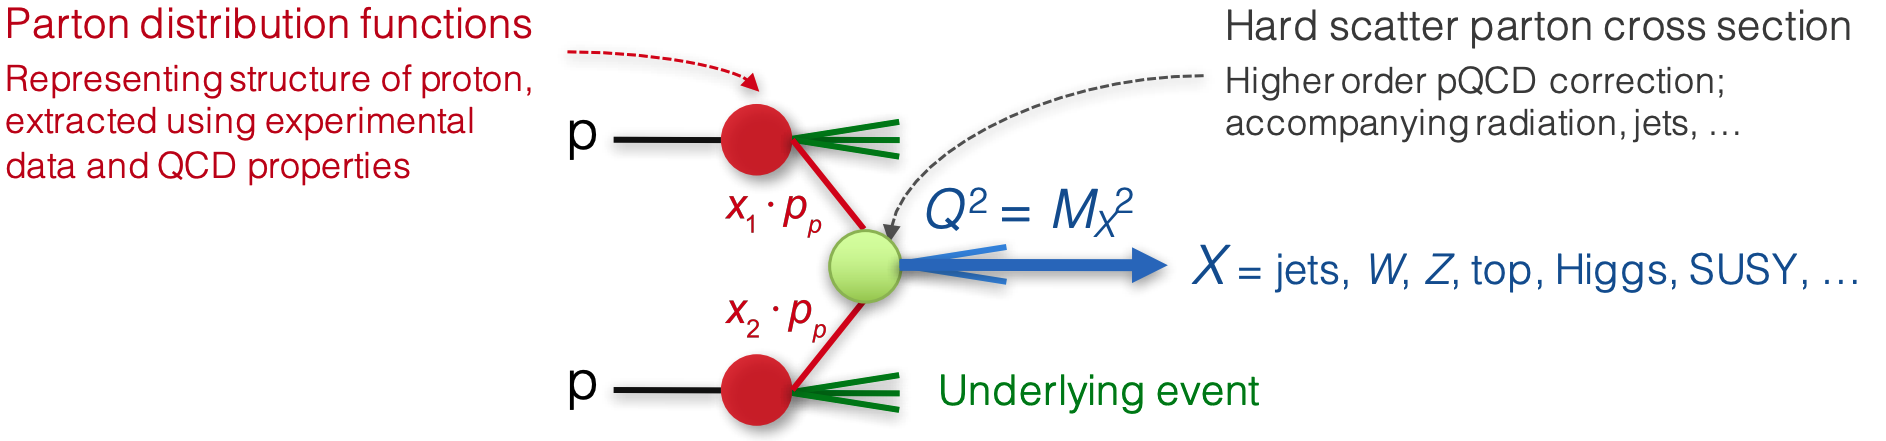
\includegraphics[width = \textwidth]{Chapter2/ProtonProton_Phenomenology}
	\caption{Simplified view of a $\Pproton \Pproton$ collision \cite{Hoecker:2016vvy}.}
	\label{fig:Chap2:ProtonProton_Collision}
\end{figure} 


%%%%%%%%%%%%%%%%%
%         Underlying Event         %
%%%%%%%%%%%%%%%%%
\subsection{Underlying event}
\label{sec:Chap1:PhenoOfPP:UE}
The Underlying Event (UE) encapsulates all what is seen from a collision that not directly comming
from the primary hard scattering process. This encompasses elements such as beam-beam remnants, 
multiple parton interactions (MPI) within a single collision, and initial and final state radiation (ISR/FSR). 
Typically, the UE have lower \pT than the main process.
A precise modelling of the UE is crucial for conducting successful experimental studies because
this soft interaction may affect the high-\pT measurements.
This is because it allows for a clear differentiation between the direct products 
from hard scattering and the rest of the event. \pablo{Maybe copy the Figure from Galo or Florencia thesis.}




%\cite{ATLAS:2010arf}
%%%%%%%%%%%
%               Data          %
%%%%%%%%%%%
\section{Data}
\label{sec:Chap3.1:Data}
\begin{itemize}
	\item How is data collected in ATLAS? DAQ
	\item Pileup (differentiate LHC pileup from ATLAS pileup during Run 2)
	\item What are triggers
\end{itemize}



%
% ATLAS Analysis model
%
\subsection{ATLAS data model}
\label{sec:Chap3.1:Data:Model}
ATLAS implements a standardised data format for reconstruction and analysis, 
supported by a data reduction framework, to generate prefiltered samples\footnote{A 
sample is a collection of events, a dataset.} for 
physics groups in a production environment. This framework facilitates the reuse 
of tools by physics groups at local levels. \cite{Buckley:2015tjh} %\cite{Brun:1997pa}

The primary data format used in ATLAS is ROOT\cite{Brun:1997pa}, which connects the reconstructed 
objects to the analysis stage. For Run 2, a novel data model was introduced, combining the advantages 
of rapid retrieval of event groups and optimised storage utilisation. In many physics analyses, intermediate-sized
 data products play a pivotal role in the early stages of the analysis workflow. These data formats are 
 typically derived directly from the preserved output of the reconstruction process, referred to as 
 Analysis Object Data (AOD) within ATLAS. Such formats exhibit common characteristics, including:
 
 \begin{enumerate}
 	\item Central Production: These data products are generated centrally for both experimental data and simulated events. 
		Their size is typically ranging from one hundredth to one thousandth of the original input data size.

 	\item Analysis Focus: AODs are specifically designed to cater to the requirements 
		of a particular analysis or a group of related analyses that share similar characteristics 
		(for instance, having the same final state objects).

 	\item Calibration and Selection: During their creation, AODs incorporate essential calibrations and 
		object selections. These calibration schemes are often shared among different physics 
		groups to ensure consistency.

  	\item Comprehensive Information: AODs encompass all the necessary information to 
		facilitate essential operations on reconstructed objects, such as smearing, scaling, 
		selection, and calibration. They also incorporate the systematic uncertainties associated 
		with these operations, collectively known as combined performance operations in ATLAS.

 	\item Reproduction and Accessibility: These intermediate data products are typically 
		reproduced 10-12 times per year. However, they are frequently accessed by 
		analysis teams, with multiple reads per week, to perform subsequent analyses 
		and investigations.


 \end{enumerate}
 By adhering to these characteristics, the AODs within ATLAS streamline the 
 analysis process, enable efficient data handling, and provide a comprehensive foundation 
 for performing various performance operations and systematic uncertainty evaluations on 
 reconstructed objects.
 
ATLAS employs various data reduction operations to streamline the analysis process.
These reduction operations are categorised as follows:
\begin{itemize}
	\item Skimming: This operation involves the removal of entire events based on specific 
		criteria related to the characteristics of the event. Events that do not meet the defined 
		criteria are excluded from further analysis.
	
	\item Slimming: Slimming involves the uniform removal of variables\footnote{A 
		variable is a property of the event or of one of its constituents (‘feature’ in
		machine learning)} within a particular type of 
		object across all objects and events. The same set of variables is eliminated for every 
		instance of the object, ensuring consistency in the data reduction process.
	
	\item Thinning: Thinning focuses on the removal of individual objects within an event based on 
		predetermined criteria associated with the properties of the object. For example, objects
		failing to satisfy certain kinematic requirements may be discarded.

	\item Augmentation: Augmentation entails the addition of supplementary information during the 
		data reduction operation to enhance the analysis capabilities. This augmentation is typically
		done in two ways:
		\begin{itemize}
			\item Adding new reconstructed object containers. For instance,  jets made with a modified algorithm.
			\item Decorating existing objects with extra variables. For example, the results of object selection by 
				combined performance tools such as ''this is a good muon''.
		\end{itemize}
\end{itemize}
% Good source: https://indico.cern.ch/event/472469/contributions/1982677/attachments/1220934/1785823/intro_slides.pdf

The flow of the data model, as depicted in Figure \ref{fig:Chap3:Analysis_data_model_ATLAS}, 
involves the use of the derivation framework for data reduction. Within this framework, intermediate 
data products are generated by selectively removing or adding information to the reconstruction output 
(i.e. AOD), while preserving the underlying structure and event data model of the original AOD. 
The analysis framework serves as the final component of the model, providing physicists with 
the means to access the derived data products, apply various combined performance tools, and 
generate the ultimate small NTuples. These NTuples serve as the basis for creating plots and 
conducting subsequent statistical analyses. In other words,  the AODs are too big to analyse directly 
and hence, the derivation framework reduces them to create the various DAODs (also known as derivations). 
DAODs are still made of xAOD objects, but are much smaller. 
This data model is implemented within
the  ATLAS software framework, Athena\footnote{Athena is the framework used for all pre-analysis data processing; it can also be
used for physics analysis.}.


\begin{figure}
 	 \centering
 	  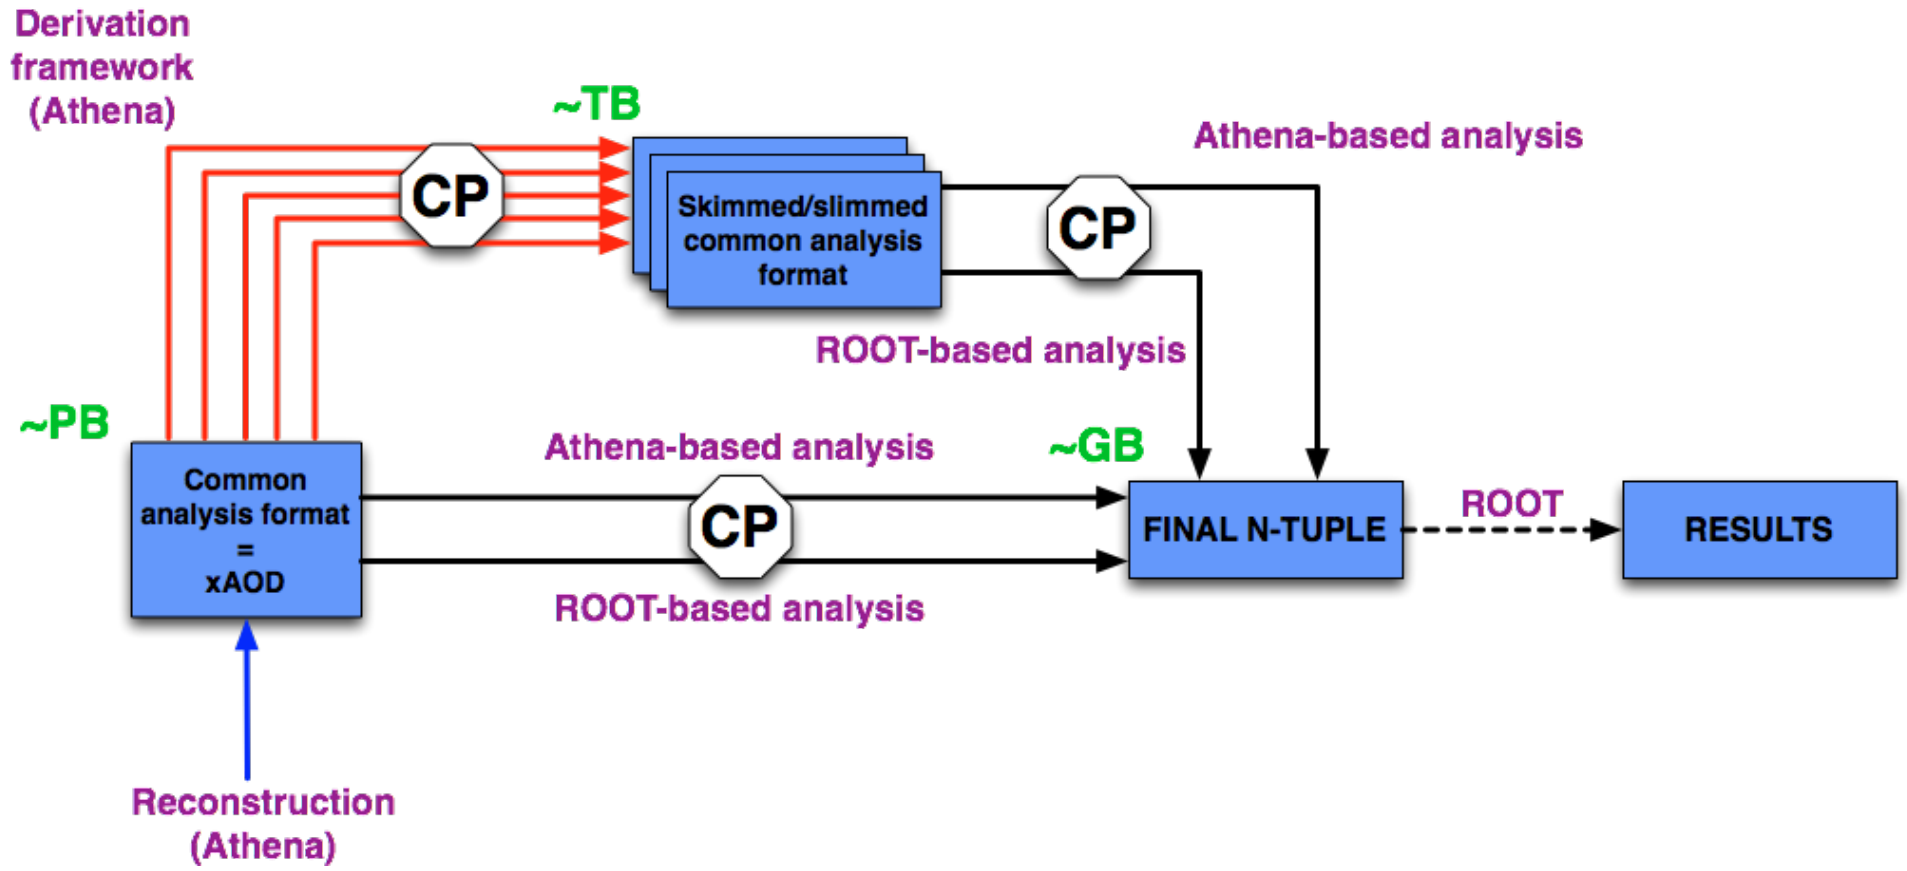
\includegraphics[width = 0.8\textwidth]{Chapter3/ATLAS_Run_2_Analysis_model}
	  \caption{Analysis model employed in ATLAS during Run 2. The scheme illustrates the transformation 
	  of the reconstruction output, known as AOD, through the derivation framework. This process results in 
	  the generation of multiple streams of Derived Analysis Object Data (DAOD). The original AOD and the 
	  derived DAOD possess compatible data models, allowing the analysis software to seamlessly use 
	  either format as input \cite{Brun:1997pa}. In this Figure CP stands for Combined Performance groups}
	\label{fig:Chap3:Analysis_data_model_ATLAS}
\end{figure}



%
% Lumi
%
\subsection{Delivered luminosity}
\label{sec:Chap3.1:Data:DeliveredLuminosity}
\pablo{This was moved from Chapter \ref{chap:ATLAS}. Adapt.}\\
The cumulative luminosity delivered by LHC to ATLAS during the Run-2 per year is shown in Figure \ref{fig:Chap2:intlumivsyear}. In 
Figure \ref{fig:Chap2:intlumivstimeRun2DQall}, the total Run-2 cumulative luminosity is presented differentiating between the delivered
 and recorded luminosity and showing that almost all delivered events are considered to be good data quality. 
 The delivered luminosity accounts for the luminosity given from the start of stable beams until the LHC requests ATLAS to put the detector in a safe standby %Reescribir este párrafo
 mode to allow a beam dump or beam studies. The recorded luminosity reflects the DAQ inefficiency, as well as the inefficiency of the 
 so‐called ``warm start'': when the stable beam flag is raised, the tracking detectors undergo a ramp of the high-voltage and, for the 
 pixel system, turning on the preamplifiers.
The All Good Data Quality criteria require all reconstructed physics objects to be of good data quality \cite{ATLAS:2019fst}. 

\begin{figure}
 	 \centering
 	  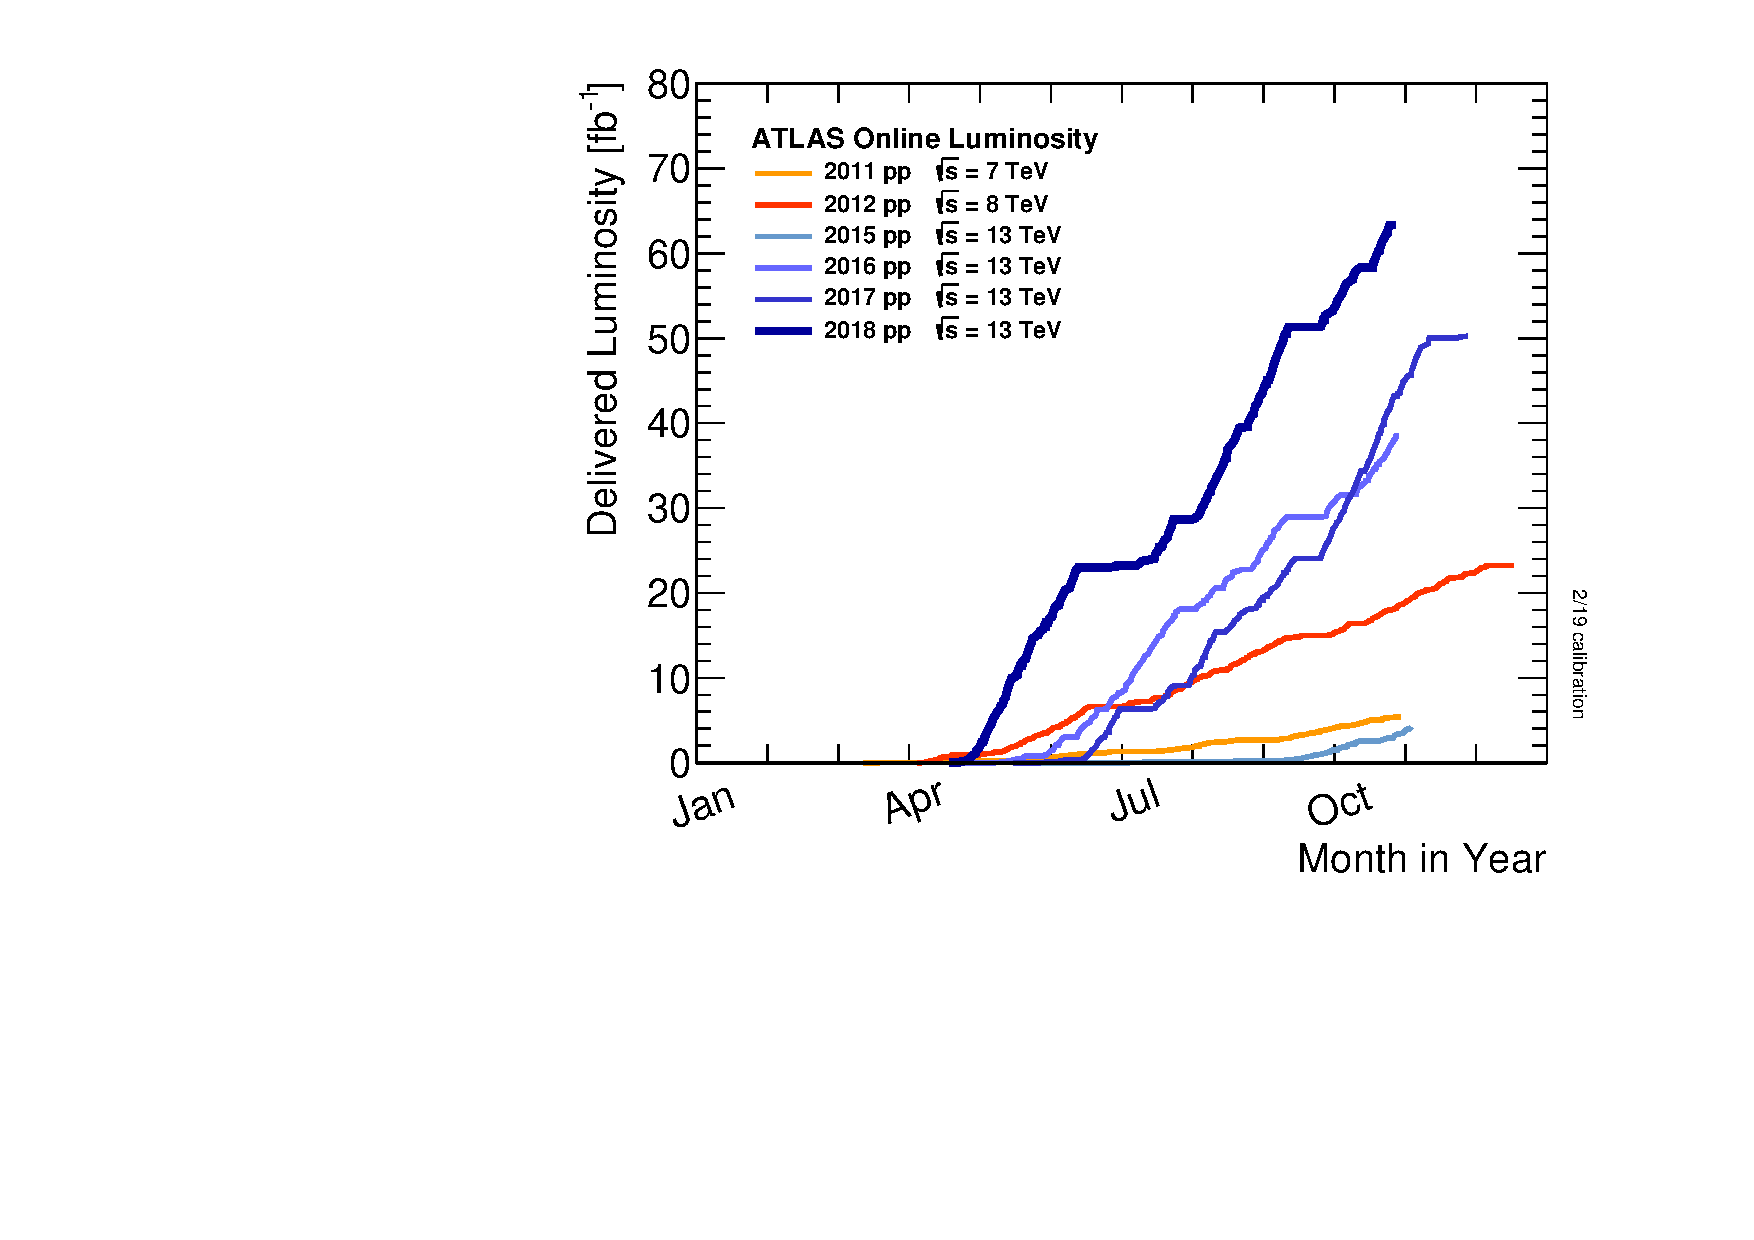
\includegraphics[width = 0.9\textwidth]{Chapter2/intlumivsyear}
	  \caption{Cumulative luminosity versus day delivered to ATLAS during stable beams and for high energy $\Pproton\Pproton$ collisions.}
	\label{fig:Chap2:intlumivsyear}
\end{figure}

\begin{table}[]
%\centering
\begin{tabular}{lllll}
\toprule
Year                                     							& 2015	& 2016 	& 2017 	& 2018 	\\ \midrule
Peak instantaneous luminosity ($\times 10^{33}\,$\lumiunits)	& 5		& 13		& 16		& 19 		\\
Total delivered integrated luminosity (fb$^{-1}$) 			& 4.0  	& 38.5 	& 50.2 	& 63.4 \\
\bottomrule
\end{tabular}
\caption{Peak luminosity and total integrated luminosity delivered by the LHC at $\CM = 13\,$TeV in Run-2 per year \cite{ATLAS:CONF:2019:021}. } 
\label{tab:Chap2:LHC:LumiRun2}
\end{table}

\begin{figure}
 	 \centering
 	  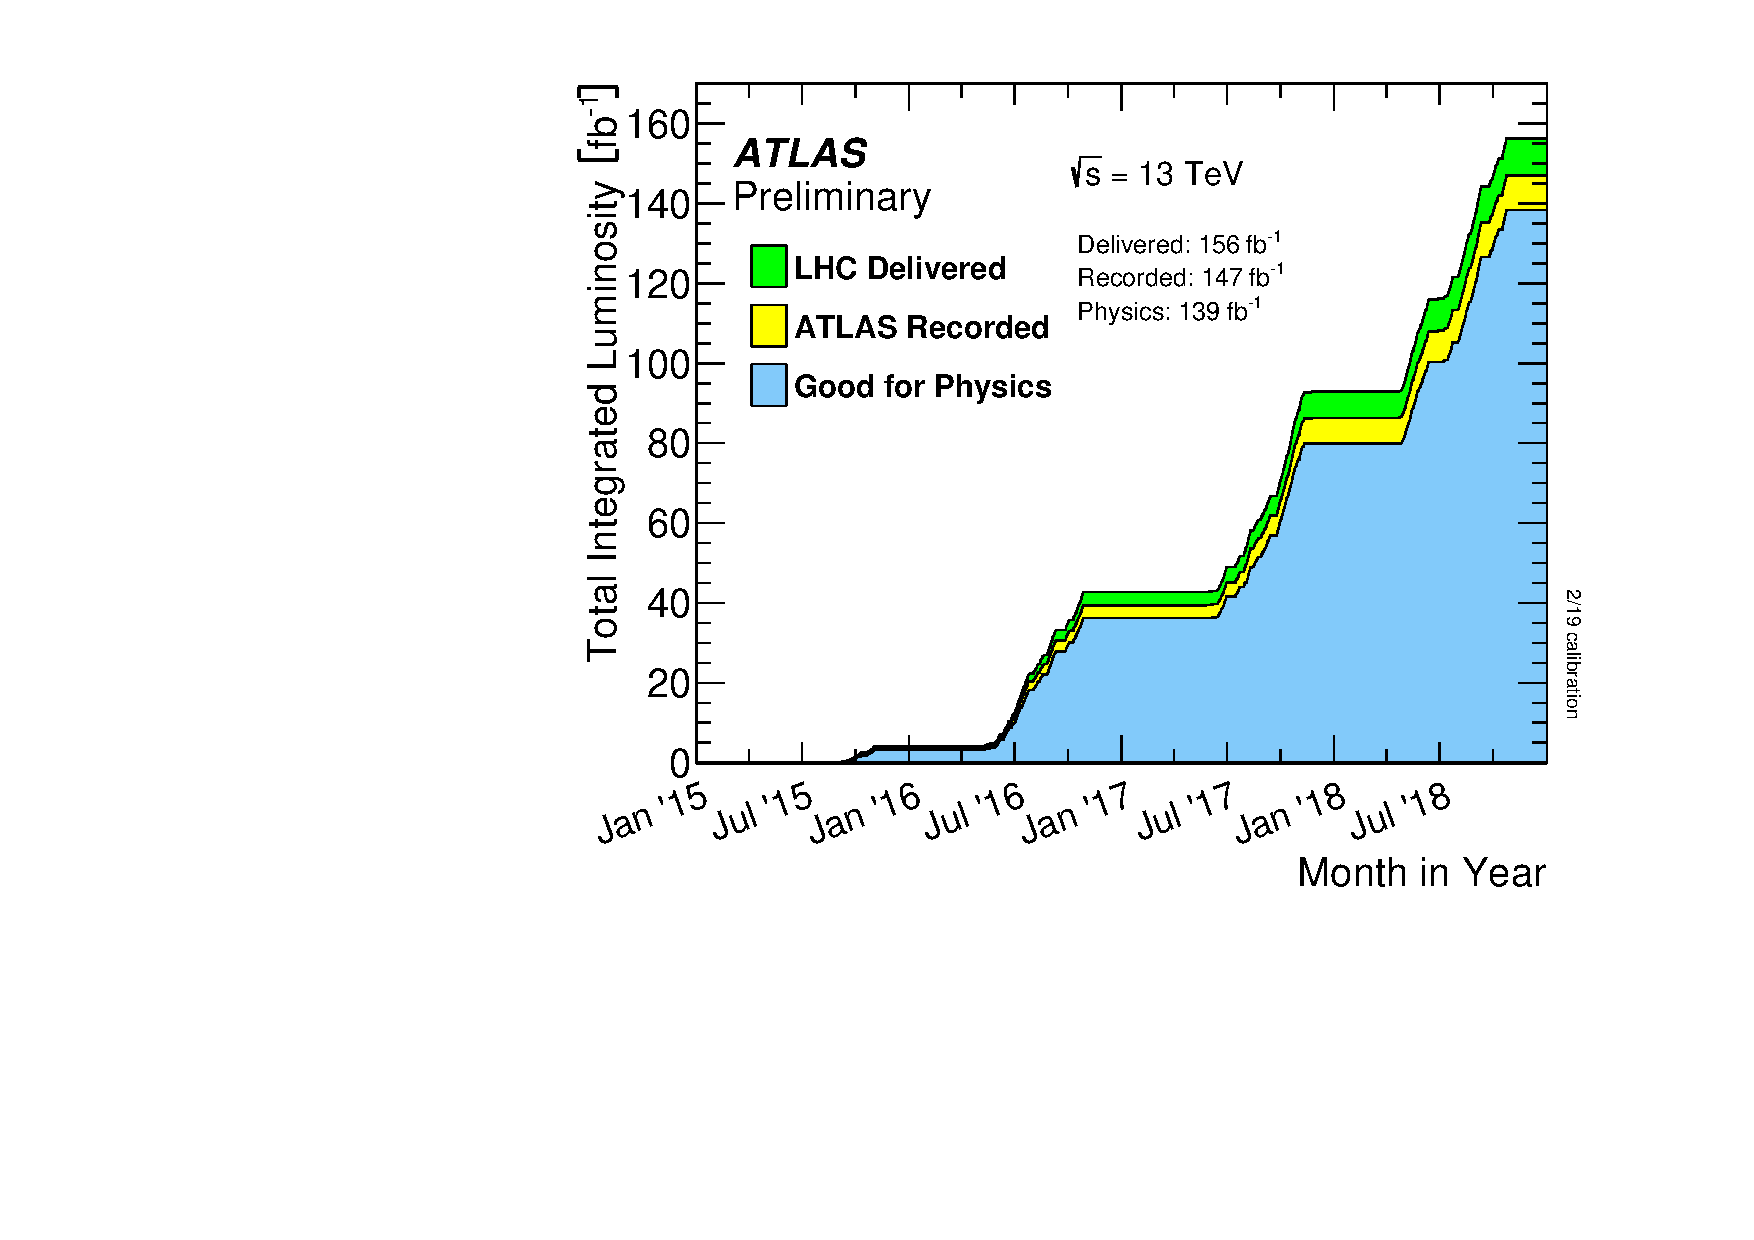
\includegraphics[width = 0.9\textwidth]{Chapter2/intlumivstimeRun2DQall}
	  \caption{Total cumulative luminosity versus time delivered to ATLAS (green), recorded by ATLAS (yellow) and certified to be good quality data (blue) during stable beams for $\Pproton\Pproton$ collisions at $\CM = 13$ TeV.}
	\label{fig:Chap2:intlumivstimeRun2DQall}
\end{figure}
%http://www.personal.soton.ac.uk/ab1u06/teaching/phys3002/course/13_accelerators_a.pdf


%%%%%%%%%%%
%              Pile-up        %
%%%%%%%%%%%
\subsection{The pile-up effect} 
\label{sec:Chap2:LHC:pileup}


Pile up is a challenging matter among detectors detector physics, and data acquisition and analysis.
Due to the fact that LHC collides bunches of protons instead of single protons, multiple particle interactions
occur at a single bunch-crossing\footnote{A bunch crossing is defined as the instance in which two 
collections of protons collide at the central region of the detector.}. This can result in multiple events
at the same time and several interactions
with the same detector element, thereby generating overlapping signals which may be difficult
to differentiate. This is what is called pile up.

Even though the bunches are composed by $\sim 10^{11}\,$ protons, there are only around 
$30\,$collisions per crossing with nominal beam currents. The mean number of interactions 
per bunch crossing is presented in Figure \ref{fig:Chap2:LHC:PileUp_15-18} for each year of 
Run-2.  The mean number of interactions per crossing 
corresponds to the mean of the poisson distribution of the number of interactions per crossing 
calculated for each bunch. It is calculated from the instantaneous per bunch luminosity as $<\mu> = \mathcal{L}_{bunch} \times \sigma_{inel} / f_{r}$
where $\mathcal{L}_{bunch}$ is the instantaneous luminosity per bunch, $\sigma_{inel} = 80\,$mb is the inelastic cross section of $\Pproton \Pproton$ collisions at $13\,$TeV
and $f_{r}=11.245\,$kHz is the LHC revolution frequency.


\begin{figure}
	\centering
 	 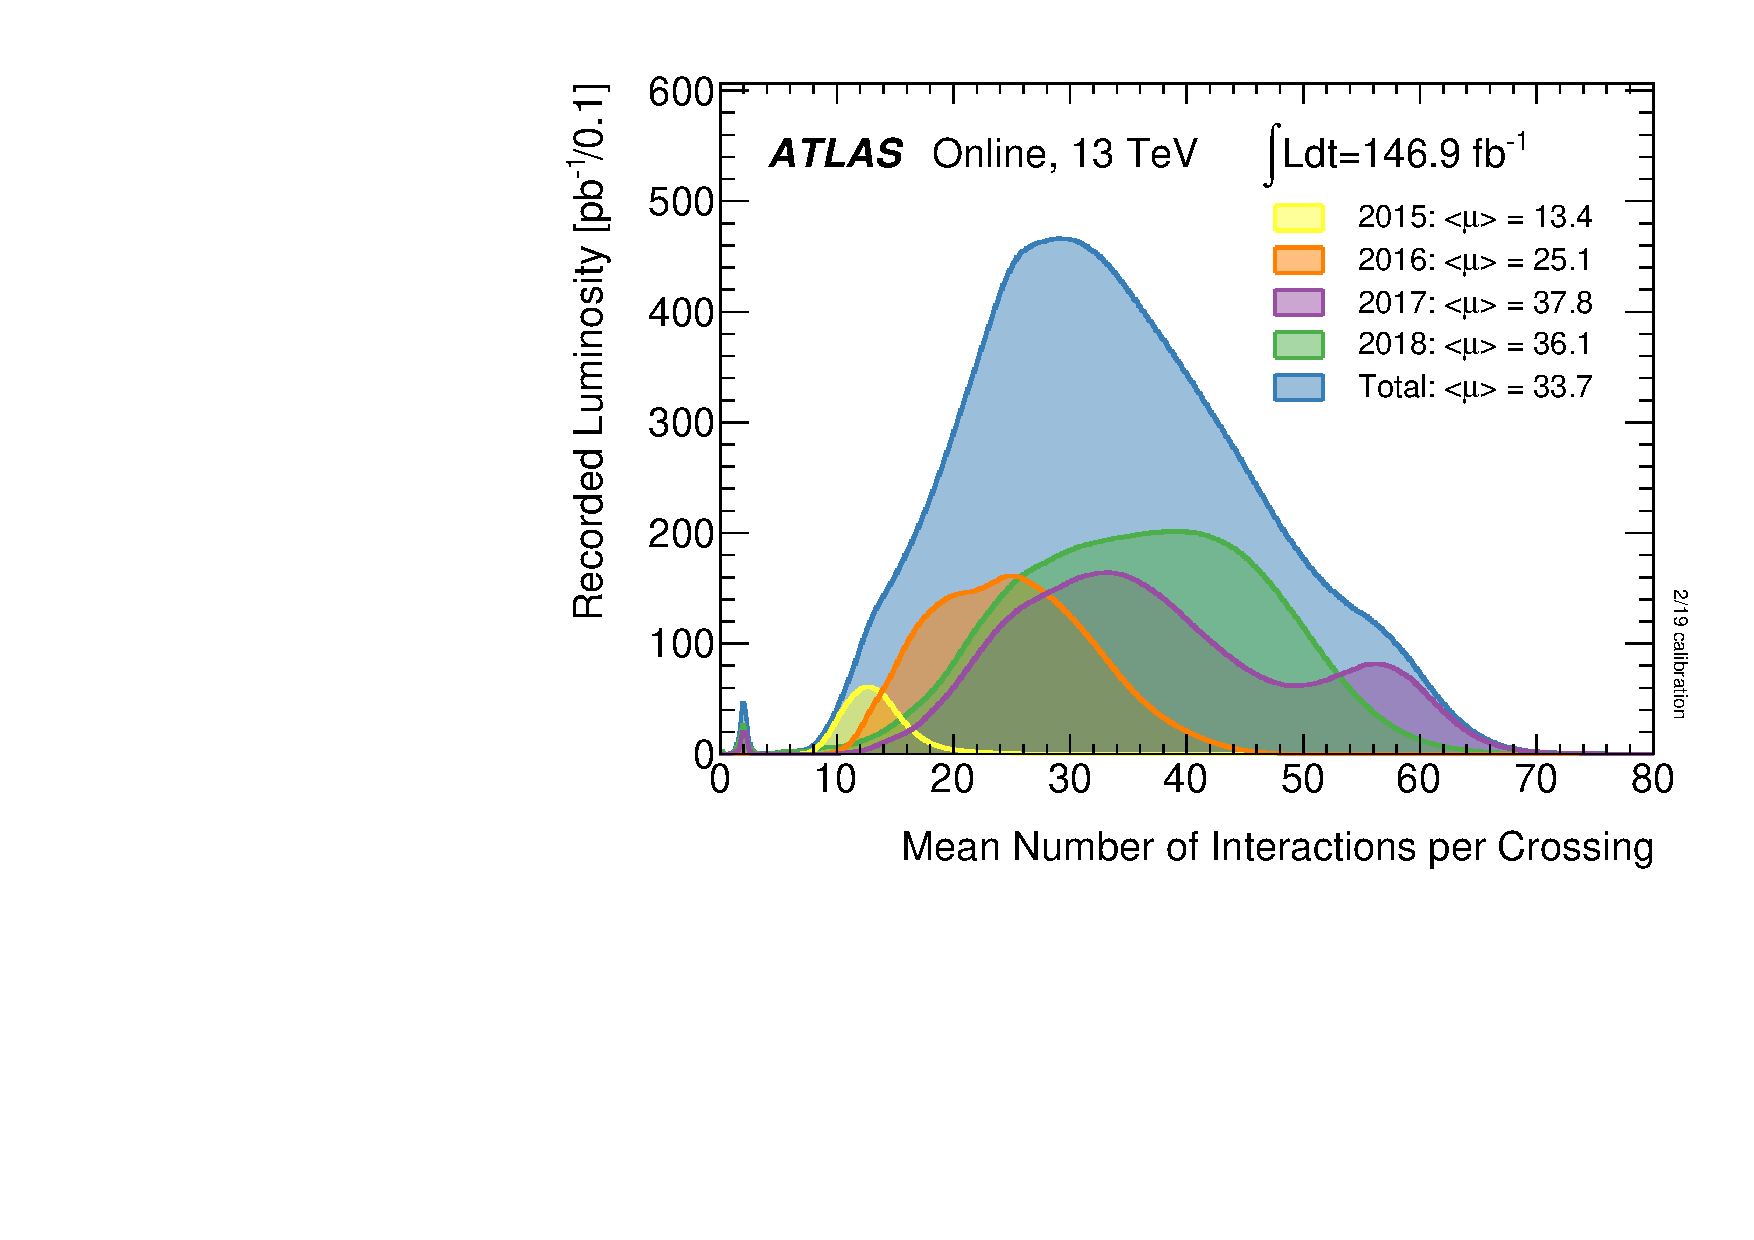
\includegraphics[width = \textwidth]{Chapter2/Pile-up_2015_2018}
	 \caption{Luminosity-weighted distribution of the mean number of interactions 
	 per crossing $<\mu >$ for Run-2 with $\Pproton \Pproton$ collisions data during stable beams at $\CM=13\,$TeV.}
	\label{fig:Chap2:LHC:PileUp_15-18}
\end{figure}

%Luminosity levelling is generally applied to reduce the number of collisions per bunch crossing 
%in the experiments when the instantaneous luminosity is too high. In 2017, when the 8b4e and 
%the 8b4e-BCS beams were used the peak luminosity exceeded the pile up limit of ATLAS and CMS \cite{steerenberg2019operation}

\pablo{Work in progress}


%%%%%%%%%%%
%             MC              %
%%%%%%%%%%%
\section{Monte Carlo}
\label{sec:Chap3.1:MC}
In order to study the physics taking place into the ATLAS detector, the signals and backgrounds in the analysis are
simulated by MC generators according to the cross sections predicted by the SM. 
The use of the MC simulations is vast and there are many different models generators and techniques. As all
 MC algorithms, these methods rely on repeated random sampling to obtain numerical results. %The underlying
%concept is based on the idea that randomness can be used to solve deterministic problems.
Since the randomness is intrinsic to the particle collision processes, a large number of events 
have to be simulated using MC technique and such a collection of events is called a MC sample.
In the context of this work, the MC generators provide a detailed simulation of the precesses from the event
generation through to output in a format which is identical to that of the true detector. 

Typically, the simulation chain can be divided into these three steps \cite{ATLAS:2010arf}:
\begin{enumerate}
    \item Generation of the events and immediate decays: %TRUTH LEVEL
    		An event generator produce the result of the collisions in terms of particles created and stores any
		stable particle expected to propagate through the detector. At this point, the geometry of the detector
		is not considered yet and only the immediate decays are taken into account. 
    \item Simulation of the detector and physic interactions:  %RECONSTRUCTION LEVEL
    		At this point, all particles from the previous step are propagated though the full ATLAS detector
		using \GEANT. This part simulates all major components and materials as well as the
		interactions of particles such us ionisation in trackers, energy deposition in calorimeters, intermediate
		decays, ration and scattering
    		
    \item Digitalisation of the energy deposits on the sensitive regions of the detector.
\end{enumerate}
% Parton and particle level at page 82: https://cds.cern.ch/record/2843747/files/TS2022_035_2.pdf

The output of the full simulation chain is an object with the exact same format as a real event registered by 
 the ATLAS DAQ system. The entire simulation chain is shown 
 in Figure \ref{fig:Chap3:SimVsReal} and compared to the path that the data follows when it is originated from an actual collision. 
 
 \begin{figure}
    \centering
    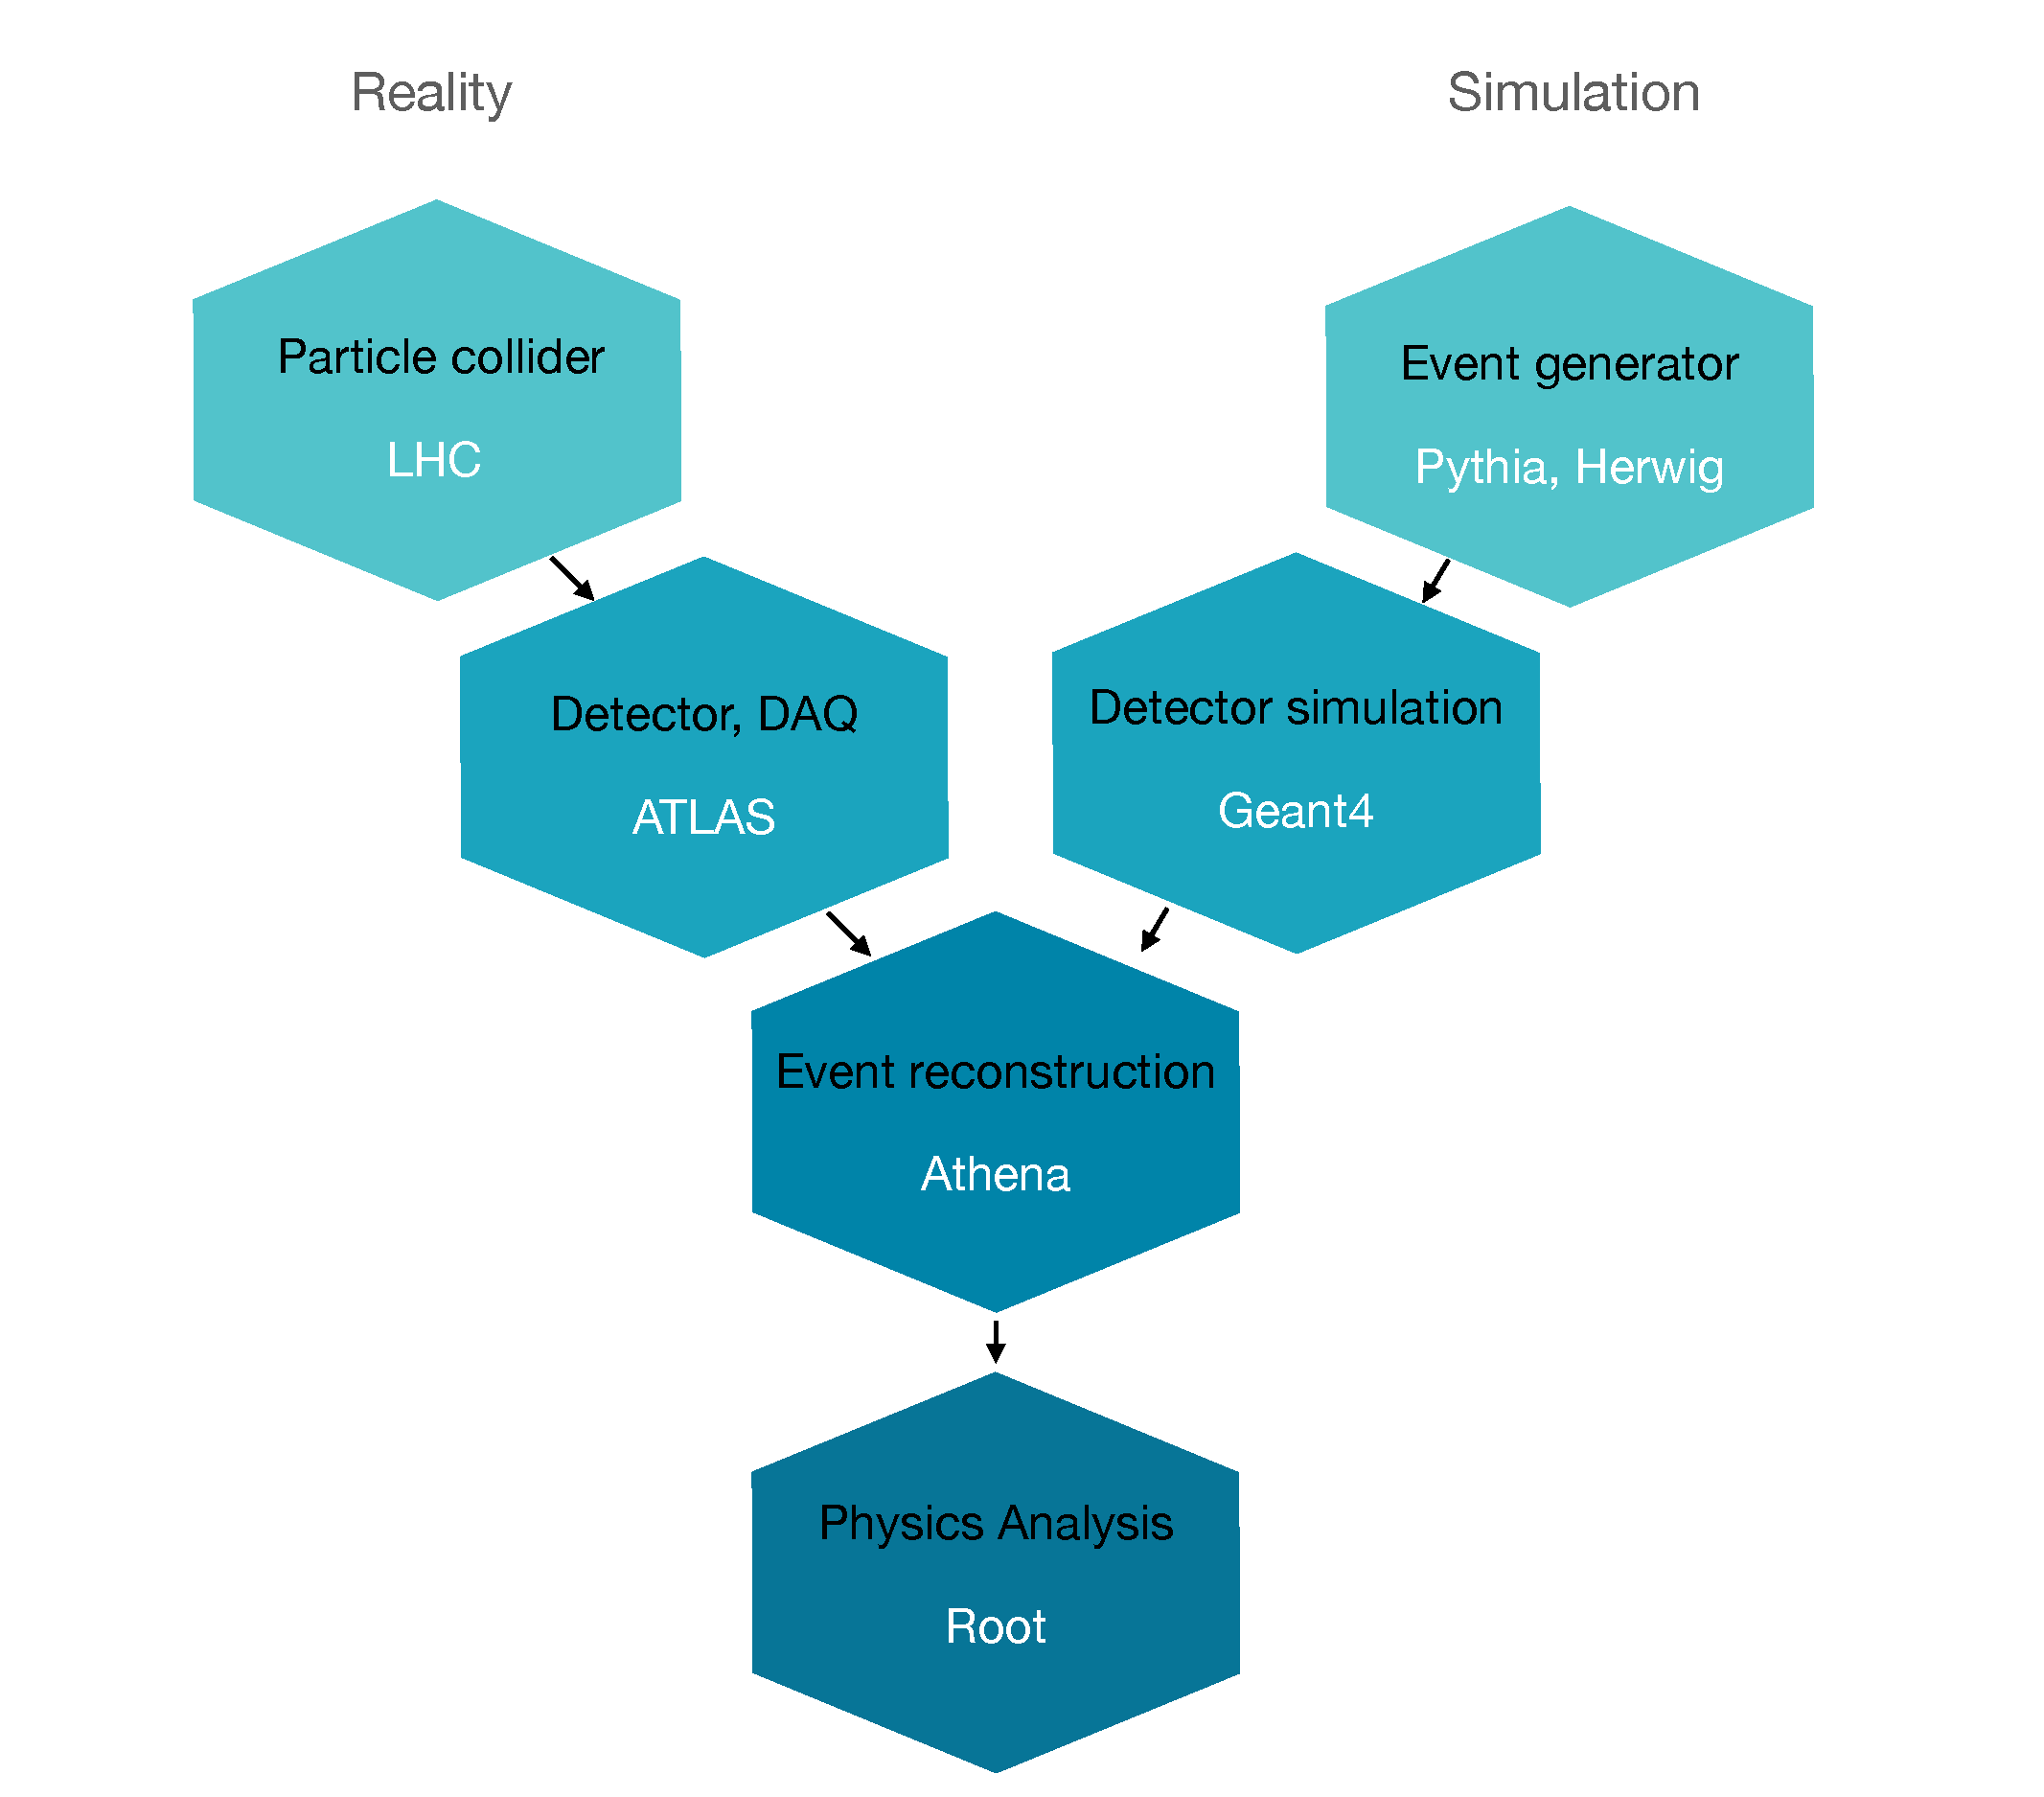
\includegraphics[width = \textwidth]{Chapter3/SimulationVSRealityChain.pdf}
    \caption{Comparison of the paths followed by data recorded by the ATLAS detector and the simulated samples.
    The format of the simulated data is the same as the recorded at each step. }
    \label{fig:Chap3:SimVsReal}
\end{figure}
 
%All implemented into ATLAS software framework, Athena.
The so called ``truth'' data is kept for each event and particle in both event generation and detector simulation. 
The truth is a history of the interactions from the generator. In the analysis presented in Chapter 
\ref{chap:Analysis_tH}, the truth information has several uses such us the determination of fake rates or the lepton 
origin assignment. An important part of the work carried during the thesis was the proper implementation of the truth 
information at generator level within Athena.


%\url{https://inspirehep.net/literature/856179}
%https://www.hep.ucl.ac.uk/~campanel/Post_Grads/2016-2017/JMorris_HEPAnalysis.pdf
%\pablo{In this section I should describe the generalities of the MC generators and in the \ref{chap:Analysis_tH} the specifics for this analysis}



\subsection{MC simulation chain}
\label{sec:Chap3.1:MC:Steps}
% Good resource: https://cds.cern.ch/record/2845282/files/CERN-THESIS-2022-268.pdf
The generation of the simulated event samples includes the effect of multiple \(pp\) interactions per 
bunch crossing, as well as the effect on the detector response due to interactions from bunch crossings 
before or after the one containing the hard interaction. 

Every different possible process that can take place
during the collision has to be simulated separately. To ensure proper description 
of the entire phase-space, the MC samples are not generated proportionally 
to the cross section of each process because that would cause a poor
characterisation of the rare processes. Instead, a sufficient large amount of raw
events are generated for each process and, afterwards, the all events
are reweighted to match their correspondent cross-section. This is the
origin of the negative weights in the MC samples. The combination of all these 
processes provides an accurate description of the collision. 

On the remaining of Section \ref{sec:Chap3.1:MC:Steps}, 
the different steps in the event generation are described. 
Starting with the hard-scattering process, which are in
the center of the simulation of scheme, the event generation
makes use of QCD corrections.

\subsubsection{Hard scattering process}
\label{sec:Chap3.1:MC:Steps:HardScattering}
The first element int the generation of the events is the simulation of the hard scattering 
processes.
Here the matrix elements of the different processes are generated at the desired accuracy 
(LO, NLO, etc). From these elements, the cross sections of the different processes are 
computed following Equation \ref{eq:chap1:Pheno:XS}. The complexity determining the 
$\mathcal{M}$ for a particular process scales with the accuracy order. 
In Section \ref{sec:Chap2:PhenoOfPP} gives more details about how the \(pp\) interactions
are modelled.
Once the hard-scatter process is simulated, many radiative corrections have to be 
applied in the form pf parton shower (PS). 

The two most important computational frameworks for implementing NLO calculations 
to obtain $\mathcal{M}$ are \MGNLO \cite{NNPDF:2014otw} 
and \POWHEGBOX \cite{Frixione:2007vw}.
		
		
\subsubsection{Parton shower simulation}
QCD corrections must be incorporated into the hard-scattering process to account 
for additional radiations. The PS models such additional radiations up to a certain 
cutoff scale, beyond which hadronisation algorithms combine the remaining quarks 
and gluons to form hadrons. This process generates hundreds of particles with 
varying energies and momenta spanning multiple orders of magnitude.

In high-energy inelastic-collisions involving hadrons, color confinement leads to the 
production of many additional partons that ultimately form hadrons. Since fixed-order 
calculations involving these partons are not feasible in hadron-collider experiments, 
PS algorithms are employed to obtain results that approximate all higher-order corrections 
due to real emissions in the hard scattering event. 


The most popular programs for PS are \Herwig \cite{Bahr:2008pv}, 
\Pythia \cite{Sjostrand:2014zea} and \Sherpa \cite{Gleisberg:2008ta}. 
The output of \MGNLO or \POWHEGBOX is used as input for the PS
generators.


 \begin{figure}
    \centering
    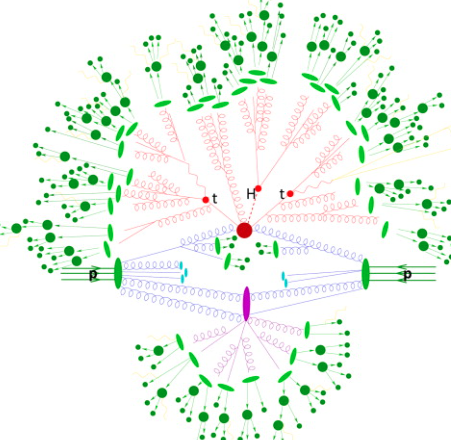
\includegraphics[width = \textwidth]{Chapter3/temp}
    \caption{Representation of a \ttH event as produced by an event generator \cite{Gleisberg:2008ta}. The big red blob is the hard interaction, which is followed by the decay of the Higgs boson and the two top quarks, represented by the three small red blobs. The additional QCD radiation produced is in red. The secondary interaction, in purple, occurs before the hadronisation of the final-state partons (light green). In darker green, the hadron decay is presented and in the photon radiation appears in yellow. }
    \label{fig:Chap3:ttHSimulated}
\end{figure}


\subsubsection{Soft QCD components, decays and QED radiation}
Following the evolution of the PS, the event generation process continues with the 
incorporation of soft QCD phenomena, decays of unstable particles, and QED 
radiation. This encompasses the UE (described in Section \ref{sec:Chap1:PhenoOfPP:UE}) 
generation and the hadronisation process, both of which are based on models that 
cannot be deduced from fundamental principles due to their occurrence at low scales, 
where the strong perturbation series becomes unreliable. 
%To determine the model parameters, fits to experimental data are performed, 
%and the values are compiled in various tunes of the programmes.

\pablo{Maybe it is better if the paragraphs are converted into subsubsections as well.}


\paragraph{Underlaying event simulation}\mbox{}

When a hard subprocess occurs, additional production of hadrons takes place. 
This production cannot be attributed to the showering of the coloured partons involved in the subprocess. 
The concept of UE encompasses various phenomena, 
including pileup reactions, MPI, and the characteristics of the soft fragments of protons.
%The UE is thought to result from collisions among partons in the 
%incoming hadrons that are not directly participating in the hard subprocess. 
The parameters used to simulate the UE must be adjusted based on experimental data.


\paragraph{Hadronisation simulation}\mbox{}

As the PS evolves, the energy and momentum of the involved
particles decrease until reaching a point in which the confinement
takes place and hadrons are formed. The hadronisation takes place
around at $1\,$GeV and converts the coloured partons into color-neutral
hadrons. The hadronisation is a non-perturbative process and, hence, 
QCD-inspired models are used to simulate it.

\paragraph{Hadron and \Ptau decay simulation}\mbox{}

The final stage before introducing the detector geometry in event generation involves the decay of unstable hadrons. 
These hadrons can be produced in excited and unstable states during hadronisation 
and can subsequently decay into lighter, stable particles that can be detected within 
the range of the detector's dimensions. Actually, a particle is considered unstable if 
its lifetime satisfies $c\tau > 10\,$mm. Given the short lifetime of the \Ptau lepton 
($2.9 \times 10^{-13}\,$s), it is also considered unstable  its decays are generated 
within the MC event simulation chain. The high complexity of modelling and implementing 
this arises from the multitude of potential particles and decay chains involved.

\paragraph{QED radiation}\mbox{}

The effects of QED radiations from charged particles are also included in the MC generators.

\subsubsection{Simulation of the ATLAS detector and  reconstruction}
The event simulation described so far describes the generation of physical 
processes based only on the theory. At this stage of the simulation chain, 
where no information about the ATLAS detector has been included yet, the
events are referred as ``truth level'' or ``particle level'' events.

In order to compare the events simulated at truth level with the real data
collected by ATLAS, the response of the detector has to be simulated. 
This includes the interaction of the many hundreds of particles present
in each event with the detector material as well as the electronic output. 

To so, the \GEANT software \cite{GEANT4:2002zbu} is used to simulate the passage of 
the generated particles through the detector. Taking into account ATLAS
geometry \GEANT simulates the effects of both, the magnetic fields and 
the detector material. Examples of this interactions are energy loss, multiple
scattering or photon conversions as well as the hits in the sensitive material.

Afterwards, the electronic signal of each detector is simulated too. This
step is known as digitalisation. The simulated digital output is used to 
reconstruct the physical objects of the MC event. This procedure is 
done identically for real and generated data, and it is described is
Chapter \ref{chap:ObjectReconstuction}. Before performing the
digitalisation, the pile up and the triggers are simulated too.

The MC events that have undergone the complete simulation chain 
are designated as ``reconstruction level'' events. Later, for the
lepton-origin assignment (Section \ref{sec:ChaptH:Sig:LepAsign})
these denominations are used when comparing the information of 
a single event at different levels.

 

\subsubsection{Pile-up simulation}
\label{chap:DataAndMC:pileup}
The effects of the pile up (described in Section \ref{sec:Chap2:LHC:pileup}) have to
be simulated as well. After the detector simulation step, this phenomenon is modelled 
by overlaying over the original hard-scattering event. To do so, \PYTHIA[8] generates
the minimum-bias events, i.e. events with low momentum transfer. The MC events are 
weighted to reproduce the $<\mu>$ observed in the data. 


\begin{comment}
\subsection{MC generators}

\pablo{Yo no metería esta sección.}

Several MC event-generator programs use the general features outlined above
to imitate the experimental data.  This thesis uses the most common generators. 
This section provides a description of these. The MC generators implemented include:

% GENERATORS:
%      MadGraph5_aMC@NLO 2.6.2
%      MadGraph5_aMC@NLO 2.3.3
%      MadGraph5_aMC@NLO 2.8.1
%      Powheg Box v2
%      Powheg Box v1
%      Sherpa 2.2.1
%      Sherpa 2.2.1-2
%      Sherpa 2.2.2
%      Sherpa 2.2.10
%      Pythia 8.186


% PARTON SHOWER:
%      Pythia 8.230
%      Pythia 8.210
%      Pythia 8.186
%      Pythia 8.245p3

\begin{itemize}
	\item \MGNLO is employed for the matrix element in the event generation
	\item \POWHEGBOX is also employed for the matrix element in the event generation
	\item \SHERPA
	\item \PYTHIA[8] takes the output of \MGNLO or \POWHEGBOX \cite{Frixione:2007vw} to simulate the PS.
				is is a C++ code. 
	\item \HERWIG for alternative PS samples
\end{itemize}
\end{comment}






%POSTAMBLE
\begin{comment}
asdf
%\end{document}
%ENDPOSTAMBLE
\end{comment}
